\appendix

\section*{Appendix}
\addcontentsline{toc}{section}{Appendix}

\newcounter{appendixcounter}
\renewcommand{\theappendixcounter}{\Roman{appendixcounter}}

%%%%%%%%%%%%%%%%%%%%%%%%%%%%%%%%%%%%%%%%%%%%%%%%%%%%%%%%%%%%%%%%%%%%%%%%%%%%%%%%%%%%%%%%%%%%%%%%

\refstepcounter{appendixcounter}

\subsection*{\Roman{appendixcounter}. Repository} \label{appendix:repository}

\addcontentsline{toc}{subsection}{\Roman{appendixcounter}. Repository}

You can find the source code, documentation, and other materials produced for this thesis in the following repositories:
\begin{itemize}
    \item Master's Thesis: \url{https://github.com/ktenman/master-thesis-ut}
    \item MMSE Prototype App: \url{https://github.com/ktenman/mmse-app}
\end{itemize}

%%%%%%%%%%%%%%%%%%%%%%%%%%%%%%%%%%%%%%%%%%%%%%%%%%%%%%%%%%%%%%%%%%%%%%%%%%%%%%%%%%%%%%%%%%%%%%%%

\refstepcounter{appendixcounter}

\subsection*{\Roman{appendixcounter}. Licence}

\addcontentsline{toc}{subsection}{\Roman{appendixcounter}. Licence}

\subsubsection*{Non-exclusive license to reproduce the thesis and make the thesis public}

I, \textbf{\authorname}, %author's name
%   \licencehint{10mm}{author's name}

\begin{enumerate}
\item
herewith grant the University of Tartu a free permit (non-exclusive license) to
reproduce for the purpose of preservation, including for adding to the DSpace digital archives until the expiry of the term of copyright,
\par
\textbf{\thesistitle}, %
%   \licencehint{10mm}{title of thesis}
\par
supervised by \supervisor. %supervisor's name
%   \licencehint{10mm}{supervisor's name}
\item
I grant the University of Tartu a permit to perform the work specified in p. 1 available to the public via the web environment of the University of Tartu, including via the DSpace digital archives, under the Creative Commons license CC BY NC ND 3.0, which allows, by giving appropriate credit to the author, to reproduce, distribute the work, and communicate it to the public, and prohibits the creation of derivative works and any commercial use of the work until the expiry of the term of copyright.
\item
I am aware of the fact that the author retains the rights specified in p. 1 and 2.
\item
I certify that granting the nonexclusive license does not infringe on other persons' intellectual property rights or rights arising from the personal data protection legislation. 
\end{enumerate}

\noindent
Konstantin Tenman\\ %author's name
\textbf{\textsl{13/08/2024}}

%%%%%%%%%%%%%%%%%%%%%%%%%%%%%%%%%%%%%%%%%%%%%%%%%%%%%%%%%%%%%%%%%%%%%%%%%%%%%%%%%%%%%%%%%%%%%%%%
\newpage
\refstepcounter{appendixcounter}

\subsection*{\Roman{appendixcounter}. Traditional Mini-Mental State Examination (MMSE)} \label{appendix:mmse}

\addcontentsline{toc}{subsection}{\Roman{appendixcounter}. Traditional Mini-Mental State Examination (MMSE)}

The following table details the tasks involved in the traditional Mini-Mental State Examination (MMSE):

\begin{table}[h!]
\centering
\caption{Traditional Mini-Mental State Examination (MMSE)}
\begin{tabular}{|p{0.3\textwidth}|p{0.6\textwidth}|}
\hline
\textbf{Task} & \textbf{Description} \\
\hline
Orientation to Time (5 points) & Assess the person's awareness of the current date and time. Questions include the date, day of the week, month, and year. \\
\hline
Orientation to Place (5 points) & Assess the individual's awareness of their current location. Questions include the type of building, the floor, the city, etc. \\
\hline
Registration of Three Objects (3 points) & Test immediate memory and attention by having the person repeat three unrelated objects. \\
\hline
Attention and Calculation (5 points) & Evaluate attention and working memory by having the person subtract 7 from 100 and continue subtracting 7, or spell "world" backward. \\
\hline
Recall of Three Objects (3 points) & Test the ability to store and recall information after a short delay by having the person recall the three objects from the registration task. \\
\hline
Naming (2 points) & Test semantic memory and language production by having the person name two objects (like a pencil and a watch). \\
\hline
Repetition (1 point) & Test language production and verbal comprehension by having the person repeat a phrase like "No ifs, ands, or buts". \\
\hline
Three-Stage Command (3 points) & Assess the ability to understand and follow complex instructions by having the person follow a three-step command. \\
\hline
Reading (1 point) & Test reading comprehension by having the person read and follow a written command like "Close your eyes". \\
\hline
Writing (1 point) & Assess writing ability by having the person write a sentence. \\
\hline
Drawing (1 point) & Assess visuospatial abilities by having the person copy a complex diagram like two intersecting pentagons. \\
\hline
\end{tabular}
\label{tab:traditional-mmse}
\end{table}

%%%%%%%%%%%%%%%%%%%%%%%%%%%%%%%%%%%%%%%%%%%%%%%%%%%%%%%%%%%%%%%%%%%%%%%%%%%%%%%%%%%%%%%%%%%%%%%%


\newpage
\refstepcounter{appendixcounter}
\subsection*{\Roman{appendixcounter}. System Architecture Overview} \label{appendix:system-architecture}
\addcontentsline{toc}{subsection}{\Roman{appendixcounter}. System Architecture Overview}
\begin{figure}[h]
\centering
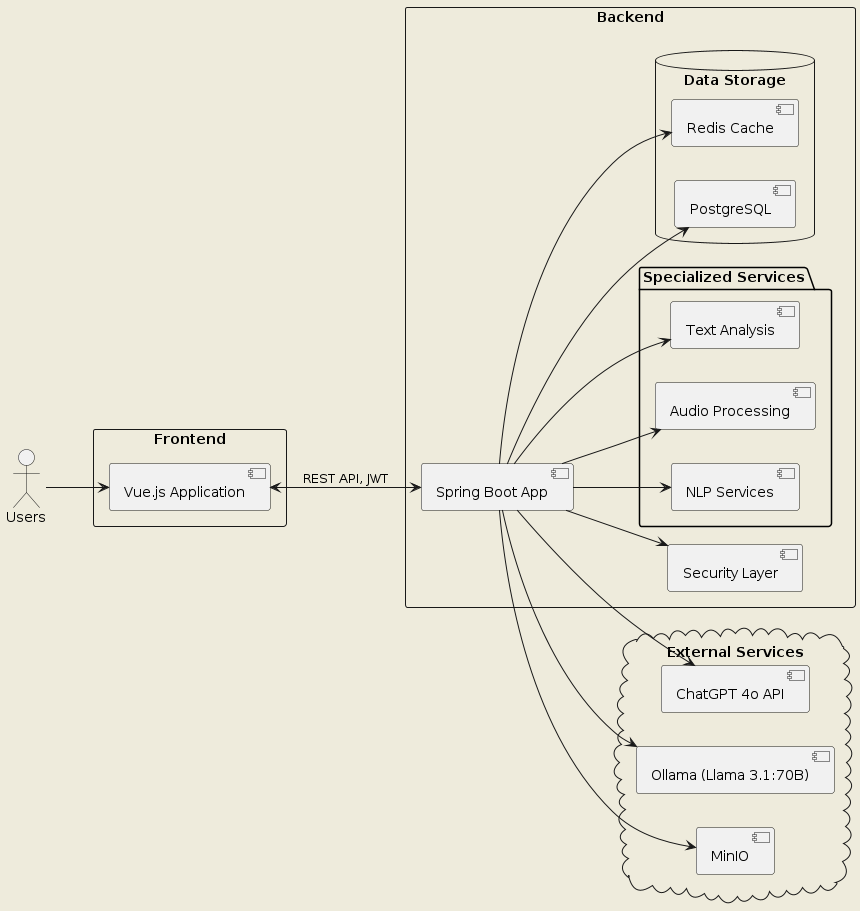
\includegraphics[width=0.95\textwidth]{system_architecture_overview.png}
\caption{High-level architecture diagram of the AI-Powered Web-based MMSE Application, illustrating main components and their interactions}
\label{fig:high-level-architecture}
\end{figure}


\newpage
\refstepcounter{appendixcounter}
\subsection*{\Roman{appendixcounter}. Participant Consent Form} \label{appendix:concent}
\addcontentsline{toc}{subsection}{\Roman{appendixcounter}. Participant Consent Form}

{\small % Reduce font size for the entire form
\section*{\small Participant Consent Form for AI-Powered and Traditional MMSE Tool Testing}
\vspace{-0.3cm}
\noindent
You are invited to participate in a research study to evaluate both the AI-powered MMSE tool and traditional paper-based MMSE tests. The purpose of this study is to assess the usability, accuracy, and effectiveness of the AI-powered tool in comparison to traditional methods of cognitive assessment. Your participation will involve completing a series of cognitive assessments using both the AI-powered MMSE tool and traditional paper-based MMSE tests.

\vspace{0.2cm}
\noindent
\textbf{Confidentiality and Data Protection}
\vspace{-0.2cm}
\begin{itemize}
    \setlength{\itemsep}{0pt}
    \item Your participation in this study is voluntary, and you may withdraw at any time without penalty.
    \item All data collected during the study will be kept confidential and will be anonymized.
    \item The data will be used solely for the purposes of this research and will be removed from our records after the analysis is complete.
    \item Your identity will not be revealed in any reports or publications resulting from this study.
\end{itemize}

\vspace{0.2cm}
\noindent
\textbf{Consent}
\vspace{-0.2cm}
\begin{itemize}
    \setlength{\itemsep}{0pt}
    \item I understand the purpose of this study and what is expected of me as a participant.
    \item I understand that my participation is voluntary and that I may withdraw at any time without penalty.
    \item I understand that my data will be kept confidential and will be removed after the analysis is complete.
    \item I understand that I will be completing both AI-powered and traditional paper-based MMSE tests.
    \item I agree to participate in this study.
\end{itemize}

\vspace{0.2cm}
\noindent
\textbf{Participant's Signature:} \underline{\hspace{8cm}}

\noindent
\textbf{Participant's Printed Name:} \underline{\hspace{8cm}}

\noindent
\textbf{Date:} \underline{\hspace{8cm}}

\vspace{0.2cm}
\noindent
\textbf{Researcher's Contact Information}

\noindent
If you have any questions or concerns about this study, please contact:

\begin{tabbing}
\hspace{2cm} \= Name: \hspace{0.5cm} \= [Your Name] \\
\> Email: \> [Your Email] \\
\> Phone: \> [Your Phone Number]
\end{tabbing}
} % End of small font size


\newpage
\refstepcounter{appendixcounter}

\subsection*{\Roman{appendixcounter}. Writing Workflow} \label{appendix:writing-workflow}

\addcontentsline{toc}{subsection}{\Roman{appendixcounter}. Writing Workflow}

The author utilized a comprehensive set of tools and environments, which are documented here to illustrate the workflow.

The writing process relied on \LaTeX{}, a robust document preparation system that emphasized content over formatting. IntelliJ IDEA and Overleaf were the primary development environments, with Overleaf selected for its collaborative and template management features.

Version control was managed with Git, with GitHub hosting the remote repository containing the \LaTeX{} source files, MMSE prototype app code, and associated documentation, as detailed in Appendix~\ref{appendix:repository}. GitHub Copilot assisted with code completion and debugging.

AI tools, including ChatGPT, Grammarly, and Claude AI, were employed to summarize, rewrite, contextualize, and refine content. Grammarly enhanced language precision. Diagramming was done using PlantUML and draw.io, which facilitated the creation of precise and standardized diagrams, with draw.io particularly useful for more complex, interactive, and visually detailed diagrams.
